\documentclass[12pt]{article}
\usepackage{fullpage}
\usepackage{svg}
\usepackage{float}
\usepackage{listings}
\usepackage{setspace}
\usepackage{url}
\usepackage{natbib}
\parskip 7.2pt
\usepackage[margin=1in,footskip=0.25in]{geometry}
\widowpenalty10000
\clubpenalty10000
\setlength\parindent{0pt}
\setlength\parskip{7mm}
\setlength\intextsep{10mm}
\setlength{\textfloatsep}{15mm}
\captionsetup{width=0.90\textwidth}
\definecolor{color_gray}{rgb}{0.5,0.5,0.5}
\lstset{
  backgroundcolor=\color{white},   % choose the background color; you must add \usepackage{color} or \usepackage{xcolor}
  basicstyle=\ttfamily,        % the size of the fonts that are used for the code
  breakatwhitespace=false,         % sets if automatic breaks should only happen at whitespace
  breaklines=true,                 % sets automatic line breaking
  belowskip=3em,
  aboveskip=3em,
  prebreak={},
  postbreak=\raisebox{0ex}[0ex][0ex]{\ensuremath{\color{red}\hookrightarrow\hspace{100pt}}},
  captionpos=b,                    % sets the caption-position to bottom
  commentstyle=\color{color_gray},    % comment style
  escapeinside=\`\`,
  extendedchars=true,              % lets you use non-ASCII characters; for 8-bits encodings only, does not work with UTF-8
  frame=single,                    % adds a frame around the code
  keepspaces=true,                 % keeps spaces in text, useful for keeping indentation of code (possibly needs columns=flexible)
  keywordstyle=\color{blue},       % keyword style
  language=C,                 % the language of the code
  numbers=left,                    % where to put the line-numbers; possible values are (none, left, right)
  numbersep=5pt,                   % how far the line-numbers are from the code
  numberstyle=\tiny\color{gray}, % the style that is used for the line-numbers
  rulecolor=\color{black},         % if not set, the frame-color may be changed on line-breaks within not-black text (e.g. comments (green here))
  showspaces=false,                % show spaces everywhere adding particular underscores; it overrides 'showstringspaces'
  showstringspaces=false,          % underline spaces within strings only
  showtabs=false,                  % show tabs within strings adding particular underscores
  stepnumber=2,                    % the step between two line-numbers. If it's 1, each line will be numbered
  tabsize=2,                       % sets default tabsize to 2 spaces
  title=\lstname}                   % show the filename of files included with \lstinputlisting; also try caption instead of title


\begin{document}

\title{Designing a Wait-Free Multiple-Producer Single-Consumer Queue for Use in SeaOS}
\author{Daniel Bittman \\ \texttt{\small{danielbittman1@gmail.com}}\\\texttt{\small{dbittman@ucsc.edu}}\\
\large{University of California, Santa Cruz}}


\maketitle
\doublespacing
\clearpage

\begin{center}
	{\large Acknowledgments}\\
	The Storage Systems Research Center at UC Santa Cruz.\\
	Darrell Long - Advisor.
\end{center}

\clearpage

\section*{Abstract}

SeaOS is a \textsc{unix} compatible self-hosting kernel designed for simplicity and
rapid prototyping. The increasingly solid support of C11 in modern C compilers
has made it possible to replace the manually implemented atomic operations
library of SeaOS with one built into the language, thus improving simplicity
and maintainability while offering more control over memory ordering requirements.
A wait-free multiple-producer single-consumer (MPSC) circular queue was implemented using C11 atomics as the first
part of work to implement more wait-free data structures into the SeaOS kernel.
When compared to a similar queue with all threads serialized with a mutex, the
performance was much improved in all situations, especially those with a large
number of producer threads.

\clearpage
\singlespacing
\tableofcontents
\clearpage
\onehalfspacing
\listoffigures
\renewcommand{\lstlistlistingname}{List of Source Code Listings}
\lstlistoflistings
\doublespacing
\clearpage

\section{Introduction}

A common need in designing or redesigning a system or idea
is to write a prototype implementation.
This is common inside of operating system kernels which, because they are quite
complex, could easily see a modification to some part of itself while
keeping the rest of the system's functionality intact -- for example writing a new
IO scheduling algorithm without touching the virtual file system. An operating
system that is going to be used for this would need to be relatively simple
and easy to understand while
providing a familiar environment and enough existing infrastructure
for normal use. A common choice for this is the Linux kernel, which
is both \textsc{unix} compatible, and provides plenty of existing infrastructure to
be useful.

% linux too big, seaos good for prototyping
However, Linux is not designed for this kind of work. It is too big
complicated, and does not allow for a researcher to rapidly prototype a
proof of concept and iron out flaws in their ideas. As an alternative solution,
I have been developing
an operating system designed for this rapid prototyping. SeaOS is a \textsc{unix} compatible
operating system designed to be as simple as possible without giving up
performance. It is designed with this kind of rapid prototyping in mind,
designed to be portable, and designed to be easy to understand. Clocking
in at just around 12,000 lines of code for the core kernel (not including drivers), it is much easier to quickly understand and start coding for than
Linux, which is at 300,000 lines of code and rising \cite{linuxsource}. 

The SeaOS kernel is self-hosting, modular, and cleanly designed and written. It is
very easy to understand, while providing good stability and performance. The design
of the code would provide a good introduction to real-world kernel programming
for students. It runs on 64-bit x86 processors, supports SATA drives, can read EXT2
filesystems, and supports a nearly complete basic \textsc{unix} userland. The source code
is available online, and hosted on github\footnote{For more information, see
the project webpage at \url{http://dbittman.github.io/seaos/index.html}.}.

\subsection{C11 in SeaOS}
% seaos <- C11; C11 adds useful shit
Because SeaOS has existed for some years, the C programming language has
evolved throughout the project. C11, the most recent standard for the C programming language released
in 2011 \cite{iso-c11}, has been slowly gaining support by gcc as their team implements more and more
features defined by the standard. C11 adds a number of useful features, including the ability to specify
memory alignment of variables, some rudimentary generics, a built-in threading library\footnote{This is not currently
implemented on most compilers.}, and,
most notably,
a language-level atomic operations library. I updated the build tools for SeaOS
and enable C11 when compiling the kernel, allowing me to take advantage of those features.
As part of this, I replaced the old atomic operations library I had written in assembly
with those provided by C11. This grants me more features and control over the
use of atomics in SeaOS, while lifting the burden of maintaining my own atomics library.

This heavy set of modifications is made possible due to the simplicity of SeaOS's design. Other kernels, such
as Linux, have decided to stick with their current atomics implementations. In early
2014, the Linux kernel developers wrote about how they did not plan to switch to
using C11 atomic operations, citing the difficulty in modifying a lot of the code
base, especially considering that their current implementation provided most of the
features that C11 does \cite{linux-no-c11}. However, the SeaOS atomics implementation was not as complete
and the code base is much smaller and simpler, making the switch to C11 easier.

\subsection{Wait-Free Data Structures}

% multithreaded programming hard; common sol. locks, but that sucks
A common problem in multi-threaded programming is how to deal with shared mutable
data. Simple variables like integers can be made atomic, but more complex data
structures require more synchronization in order to safely share them between
threads. A common solution is to simply put a lock around the data structure,
preventing more than one thread from accessing it at any one time. This solves
the problem of concurrent access to the shared data structure, but it seriously
hurts performance and scalability to many threads, as they all have to fight
to acquire the lock before they can make any progress.

% wait-free

Another solution is to design the data structures such that its operations
do not require threads to be serialized. A data structure is called wait-free
if a thread will complete an operation on the data structure in a finite number
of steps, regardless of if other threads that are operating on the data structure
are blocked or interrupted in some way \cite{herlihy1991wait}. This has the advantage of both
scalability -- multiple threads may operate on the data structure simultaneously (a
mutex would violate the wait-free property) -- but it is also safer to use. A
thread that gets scheduled away or encounters a page fault does not obstruct
the progress of other threads. This is especially useful in kernel space, as it
means that such data structures are safe to use inside interrupt handlers without extra
work done for synchronization.

% implement into seaos, MPSCQ
With the addition of the new atomics library, I have started implementing
wait-free data structures into SeaOS. The kernel currently provides a number of common
data structures such as linked lists, queues, heaps, hash tables, etc, however they all use
locks to do thread synchronization. As a first step in this project, I have implemented a
wait-free multiple-producer single-consumer circular queue, which uses C11 atomics to
synchronize threads instead of a mutex or other locks. I have chosen this type of queue
because it is already in use in the kernel in several locations which would benefit from
improved scalability with number of threads. It is written in C and currently implemented
in userspace for testing.

Similar wait-free queue have been written about \cite{david2004single}
\cite{kogan2011wait} \cite{valois1994implementing}. However, many of these are either
for single-producer single-consumer queues (queues that only allow one thread to enqueue
and one thread to dequeue) or multiple-producer multiple-consumer queues (queues that allow
any number of threads to enqueue and dequeue). The former is too restrictive for my use case, and the
later has extra overhead from allowing multiple consumers which I do not need for my
use case. Additionally, many of these queues were written before the advent of C11, meaning
that writing such a queue in C11 gives a unique opportunity to study the C11 atomics system
and how it can be used to make performant wait-free data structures.

\section{C11 Atomics: \texttt{stdatomic.h}}

% basics of c11 atomics
C11 introduces the header file \texttt{stdatomic.h}. It provides a number of functions to do
basic arithmetic and bitwise operations, as well as more complex operations like compare and
swap (CAS). The arithmetic and bitwise operations are named as \texttt{atomic\_fetch\_\textit{operation}},
and can be called like \texttt{atomic\_fetch\_\textit{operation}(\&dest, val)}.
These functions do the specified operation on the variable
atomically (for example, \texttt{atomic\_fetch\_or} will atomically do \texttt{dest |= val}), and then return
the previous value of the variable. In addition to these operations, C11 provides \texttt{atomic\_store}, \texttt{atomic\_load}, and \texttt{atomic\_exchange}.
These allow the modification of variables without torn reads and writes, and atomically exchanging the value of
a variable with another value.

% atomic variables
Any variable may be declared as atomic by specifying the \texttt{\_Atomic} keyword in the declaration.
This will cause any normal expression involving that variable to be atomic. For example, referencing
that variable will be an atomic load, storing to the variable will be an atomic store, and incrementing
the variable will be an atomic increment. Most standard types have atomic versions defined, such as
\texttt{atomic\_int}, or \texttt{atomic\_size\_t}.

\subsection{Memory Ordering}

% C compiler reorders
When a programmer writes code in a language like C, the compiler does more than a direct translation to assembly
language. Instead, it tries to convert the unoptimized operations made by the programmer into a more efficient
order which will perform better. This optimization is very effective and lowers
the need for the programmer to micro-optimize their code, but it can make bugs more difficult to find, and concurrency harder to reason about.

% CPU reorders, example of why reordering is hard
Furthermore, the CPU takes the binary code and decides that instead of executing the instructions
exactly as the compiler generated them, it will instead execute them in a much better and more efficient order that has the same
result. This is called out of order execution. By realizing that certain instructions depend on only some of the preceding
instructions, it may be more efficient to issue memory reads out of order and do arithmetic out of order. This is,
again, great for performance, but it leaves the problem of reasoning about concurrency even worse than before.

\begin{minipage}{\linewidth}
	\onehalfspacing
\begin{lstlisting}[label={sucks},caption={Example of how reordering can affect
	the result of execution.}]
bool z = false;
int x = 0, y = 0;
void thread_A() {
	x = 1;
	while(x == 1) /* do nothing */;
	if(y == 1)
		z = true;
}

void thread_B() {
	while(x != 1) /* do nothing */;
	y = 1;
	x = 0;
}
\end{lstlisting}
	\doublespacing
\end{minipage}
These issue become clear in the example shown in Listing \ref{sucks}\footnote{Assuming that the compiler does not optimize away the loops, which it might do.}.
If these variables were atomic, then this would result in $z$ having the value \texttt{true}.
However, since they are not atomic it may
not work out that way. It would be valid for the compiler to reorder the two store operations done in \texttt{thread\_B},
or even move the conditional store in \texttt{thread\_A} to above the loop. None of those operations depend
on the ordering that they are listed in in a single threaded environment, and the variables are not atomic.
We may not have an easy way of knowing in what order the operations are actually
going to happen, and this is why reasoning about concurrency in an out of order execution environment is not easy.
It is very important, however, that it be done because of the increased performance that can be gained by reordering \cite{atomicweapons}.

% memory models, seqcst
To combat this problem, C11 defines a memory model.
A memory model is a description of how threads interact with memory. It defines allowed reordering behavior of the compiler and CPU
and the optimizations it may perform. C's memory model is sequential consistency \cite[\S 7.17]{iso-c11}. This means that the result of
an execution of a program is such that a total ordering of operations is observed for each thread. Simply put,
given a number of threads that have a list of operations that they are performing, the results will look like
some interleaving of those operations with their total order kept \cite{c11atomics}. It only asks that the programmer does not
write a data race, for if a data race is present all its guarantees are no longer valid.

% default seqcst, this is slow. allows relaxation.
The compiler is allowed to reorder non-atomic operations like it did before. However, using atomic
variables and operations adds certain restrictions. By default, atomic operations are sequentially consistent,
so memory accesses may not be reordered around them at all, and the compiler will emit instructions necessary
to make sure the CPU does not reorder them either. This, of course, removes a lot of the optimizations
that can be done by the compiler and CPU, and could cause an avoidable performance penalty should this
strictness be unnecessary. For this reason, the C11 atomics library gives the programmer the ability to
specify the memory ordering for a given atomic operation, allowing reordering to occur in specific ways \cite{iso-c11}.
This is called relaxing the atomics. The programmer takes over the burden of determining what kind of
reordering is safe, and may gain performance in doing so \cite{atomicweapons}.

% relaxed atomics in c11
Each of the atomic functions provided by \texttt{stdatomic.h} have a variant whose name ends with \texttt{\_explicit}.
These functions take as their last argument an \texttt{enum memory\_order}, which contains:

\singlespacing
\begin{enumerate}
	\item \texttt{memory\_order\_relaxed}
	\item \texttt{memory\_order\_acquire}
	\item \texttt{memory\_order\_release}
	\item \texttt{memory\_order\_seq\_cst}\\
\end{enumerate}
\doublespacing
The last of these is the default ordering, sequential consistency. The first, \texttt{relaxed}, attaches no ordering
requirements to the operation, thus allowing memory operations to be reordered around it in any way. The second
one gives an operation \texttt{acquire} semantics. This means that memory operations may not be reordered from after the
atomic operation to before it, but they may be reordered the other way. The third gives an operation \texttt{release} semantics,
which is the opposite of acquire semantics. It means that operations may not be reordered from before the operation to
after the operation, but they may be reordered the other way. A common use case of \texttt{acquire} and \texttt{release} is shown in Listing \ref{lst-acq-rel}.
Some architectures may see a significant performance increase when using these relaxed atomics.


\begin{minipage}{\linewidth}
\onehalfspacing
	\begin{lstlisting}[label={lst-acq-rel}, caption={[Example of relaxing atomics.]\doublespacing Example of relaxing atomics. Say some other thread sets the \texttt{ptr} variable to some work to be
done. Only one thread would do this work, because of the atomic exchange of the pointer. Additionally, any memory accesses between the exchange
and the add would not be able to move out before or after those instructions. However, any memory accesses made before the exchange or after the add
would be able to move inside that block of code.}]
_Atomic void *ptr = NULL;
_Atomic work_done = 0;
void thread_main() {
	while(true) {
		/* ... */
		void *work = atomic_exchange_explicit(&ptr, NULL, memory_order_acquire);
		if(work) {
			/* do work */
		}
		atomic_add_explicit(&work_done, 1, memory_order_release);
	}
}
\end{lstlisting}
\doublespacing
\end{minipage}
\section{Atomics in SeaOS}
% used to use c99, now use c11
Since the beginning of the SeaOS project, the compiler was set to compile using the C99 standard
even though C11 was the most recently released standard for the language. This was due to lack
of support for C11 in gcc at the time. Recently, however, I upgraded the toolchain to use a newer version
of gcc which supports most of the C11 features that are useful in kernel space. Now the kernel is compiled using the
C11 standard, so it may use atomics, booleans, and a number of other convenient features. I was able
to remove the older implementation of atomics, which was manually implemented in assembly,
making the code easier to maintain and granting the use of features from \texttt{stdatomic.h} which
were not available before.

% old atomics :: --fences?
Prior to the switch to C11, atomics for SeaOS were implemented inside \texttt{sea/cpu/atomics.h}.
They were mostly small functions which contained inline assembly operations (see Listing \ref{lst-atomic-add}).
Most of the uses of atomics in the code were to atomically increment of decrement variables (for
example, reference counting), and to implement mutexes and reader-writer locks. The atomic
operations that were provided were addition, subtraction, bitwise or, bitwise and, bit-test-and-set,
and full memory fences.
\begin{lstlisting}[label=lst-atomic-add, caption={[Manually implemented atomic addition.]Example atomic operation implementation (32-bit addition) without C11 atomics. Adds \texttt{amount} to the 32-bit integer pointed to by \texttt{val} and returns the old value. In C11 a similar function is already implemented.}]
uint32_t add32_atomic(uint32_t *val, int amount) {
	uint32_t prev_val;
	asm volatile("lock xadd %%esi, %0" : "=S"(prev_val)
			: "m"(val), "S"(amount) : "esi");
	return prev_val;
}
\end{lstlisting}

% kernel too locky
I had managed to get away with not implementing an atomic compare-and-swap (CAS) operation
or an atomic exchange operation, because
the code that implemented locking primitives did not need it. However, this
meant that a lot of code that could have gotten away with atomic operations for thread
synchronization fell back to over-using locks\footnote{An example of this was code
	that would destroy certain data structures in the kernel. Instead of doing an atomic
exchange to read and clear a pointer, it would lock the entire section of code.}.
Another feature that was lacking in the old atomics implementation was a lack of memory
ordering options. Every operation was done with the sequential consistency ordering.
This made it easier to reason about the code, but it could
have a performance impact on certain platforms.

\subsection{Upgrading to C11 Atomics}

% the easy stuff to switch
Fortunately, the atomics system I had designed was already very close in API to the C11 atomics
system. First, all references to \texttt{sea/cpu/atomics.h} had to be changed to \texttt{stdatomic.h}.
Second, the names of most atomic functions had to be changed. For example, \texttt{add\_atomic} became \texttt{atomic\_fetch\_add}.
The mutex and reader-writer lock implementations were re-written to be more efficient and were made to use
the new \texttt{atomic\_flag} type in C11. Atomic variables initialization were changed to use the
required \texttt{ATOMIC\_VAR\_INIT} macro\footnote{This macro does not actually do anything on x86. It is defined as
\mbox{\texttt{\#define ATOMIC\_VAR\_INIT(x) x}}.}.

% the trickier stuff to switch
A more involved set of modifications were due to a slight difference in behavior of the addition and subtraction
functions. In the old SeaOS atomics, \texttt{add\_atomic} and \texttt{sub\_atomic} would return the \textit{new} value of the
variable whereas the C11 versions return the \textit{old} value.
The reason the old versions did it that way is because there is a lot of the code that looks similar to
\texttt{if (sub\_atomic(\&obj->ref\_count, 1) == 0) \{ /* do something */ \}}, and I thought that was more readable and
clear than checking if the result was 1. However, I was not that attached to that choice, so I
updated every location which checked the return value of an atomic function to be correct for the new
C11 atomics.
Finally, there are a large number of cases where an atomic operation does not need sequential consistency.
I went over all of the code that used atomics and determined the obvious places where the memory ordering
could be safely relaxed, and relaxed them.

\section{A Wait-Free Multi-Producer Single-Consumer Queue}

As a test for a wait-free data structure in the kernel, I have written a wait-free multiple-producer single-consumer
circular queue. This will find use in worker threads where many threads may enqueue work, but only one will dequeue
and do work (for example, packet sending threads and elevator threads). It will replace an old queue data structure
inside SeaOS which uses mutexes to synchronize threads. My goal was to show that a wait-free version would have
higher performance and better scalability.

\subsection{Implementation Details}

The queue is defined as a struct as shown in Listing \ref{lst-queue}. It has two atomic integer values: \texttt{count} and \texttt{head},
and two non-atomic numeric values: \texttt{tail} and \texttt{max}. The value \texttt{max} may not change once a queue is created.
A slightly more complex definition is \texttt{void * \_Atomic *buffer}, which is a pointer to an \texttt{\_Atomic void *} -- an
array of atomic void pointers. This pointer is initialized to a zeroed array of void pointers during queue creation.

	\onehalfspacing
\begin{lstlisting}[label=lst-queue, caption={Definition of queue structure.}]
struct mpscq {
	_Atomic size_t count;
	_Atomic size_t head;
	size_t tail;
	size_t max;
	void * _Atomic *buffer;
	int flags;
};
\end{lstlisting}
	\doublespacing

The queue supports three operations: \texttt{enqueue}, \texttt{dequeue}, and \texttt{count}. \texttt{Enqueue} and \texttt{dequeue} are shown in Listings \ref{lst-enqueue} and \ref{lst-dequeue}
respectively. The \texttt{count} operation is much simpler, and is just an atomic load of the \texttt{count} field of the queue structure.

\begin{minipage}{\linewidth}
	\onehalfspacing
	\vspace{5mm}
	\begin{lstlisting}[label=lst-enqueue, caption={Implementation of \texttt{enqueue} function, with memory orderings.}]
bool mpscq_enqueue(struct mpscq *q, void *obj)
{
	size_t count = atomic_fetch_add_explicit(&q->count, 1, memory_order_acquire);
	if(count >= q->max) {
		/* back off, queue is full */
		atomic_fetch_sub_explicit(&q->count, 1, memory_order_release);
		return false;
	}

	/* increment the head, which gives us
	 * 'exclusive' access to that element */
	size_t head = atomic_fetch_add_explicit(&q->head, 1, memory_order_acquire);
	atomic_store_explicit(&q->buffer[head % q->max], obj, memory_order_release);
	return true;
}

\end{lstlisting}
	\doublespacing
\end{minipage}

When enqueueing an object, the thread must make sure to not overrun the queue.
Incrementing the count at the beginning and checking if the old value was less than
the maximum capacity ensures this. Consider the case where the queue has one available
space open, and two threads try to increment. This will result in exactly one of the
threads seeing the queue as not full, and the other seeing it as full.

The increment of count at the beginning gives the thread a guarantee that there will be
space for it to enqueue something in the buffer. Once it determines that there is space,
the thread increments the value of \texttt{head}, and stores the data in the buffer at
the old location of \texttt{head}. This is thread-safe, because the atomic increment
of \texttt{head} ensures that a thread has exclusive write access to that location in the
buffer within the context of the enqueue function.

\begin{minipage}{\linewidth}
	\onehalfspacing
	\vspace{5mm}
\begin{lstlisting}[label=lst-dequeue, caption={Implementation of \texttt{dequeue} function, with memory orderings.}]
void *mpscq_dequeue(struct mpscq *q)
{
	void *ret = atomic_exchange_explicit(&q->buffer[q->tail], NULL, memory_order_acquire);
	if(!ret) {
		return NULL;
	}

	if(++q->tail >= q->max)
		q->tail = 0;
	
	atomic_fetch_sub_explicit(&q->count, 1,memory_order_relaxed);
	return ret;
}
\end{lstlisting}
	\doublespacing
\end{minipage}

The dequeue function immediately
does an atomic exchange, setting the location in the buffer pointed to by tail to NULL. If
the old value of that location is non-null, then the tail pointer is incremented (and
wrapped around), the count decreased, and the value returned. If the old value was NULL,
then the function returns NULL to indicate that the queue is empty. This works because
of the requirement that an empty element of the array must be NULL. The enqueue function
only writes to the array at the end, which is what allows the dequeue function to
read out data. The dequeue function then exchanges the value with NULL, maintaining
the requirement.

Note that the dequeue function never checks count. A non-NULL value at the tail pointer
indicates the presence of data, and NULL value indicates empty. The value of count is only
ever used to determine if the queue is full during the enqueue operation. Also, the tail pointer
increment is non-atomic, since only one thread may ever be in the dequeue function at one
time (by definition).

It is possible for the count to be non-zero and for dequeue to return NULL. This could happen
if a producer thread increments count, and before it has the chance to actually do the
atomic store of the data, the consumer thread calls dequeue. This is acceptable, since
this indicates that the producer thread has not yet completed the enqueuing, which is
similar to the case of the queue being empty. A ``worst case'' scenario of this would
be a number of producer threads that have all enqueued data into the buffer, except for
the thread that would write to the location pointed to by the tail pointer. Then all of
the enqueued data is inaccessible until the single thread that would write to the
first location in the buffer is scheduled and completes the write. However, none of
the other threads are blocked because of this. It looks to the consumer thread as
if the producer thread have yet to enqueue work. In no way can the consumer thread
try to dequeue data that has not yet been written, so it is all still thread-safe.

\subsection{Testing Environment and Framework}
In order to do better testing and quicker
development, I wrote the queue for userspace Linux first. The queue itself is simply C11, and so should run anywhere
with a compiler that supports \texttt{stdatomic.h} and \texttt{stdbool.h}. The testing program assumes a Linux
environment with pthreads support. The current code can be found online at \url{https://github.com/dbittman/waitfree-mpsc-queue}.


Figures~\ref{fig-16} through~\ref{fig-8000} show the performance of the wait-free queue
compared to a similarly implemented queue locked with a mutex and without atomic operations.
The tests were done on a dual-socket machine with two Intel Xeon X5660 CPUs with 6 cores per
socket and two threads per core, running at 2.80 GHz. The machine had 96 GB of RAM.
The data were collected for a varying queue size (from 16 elements to 8000 elements)
by varying the number of threads and measuring time to completion. The test program
would start a timer right before kicking off the threads, and would then start $n-1$
threads as producers and one thread as a consumer. Once all the producers had completed
and the consumer had emptied the queue, the timer was stopped and the elapsed time reported.
Each test has a computed 95\% confidence level.
Every producer thread enqueued 100 items to the queue, and then exited. In the case
where the queue is full, it retried the item until it could be enqueued.

\subsection{Performance Results}
The results show excellent performance of the wait-free queue. It beats the performance of the mutex-based
queue in every way -- and by a significant margin when the number of threads is large -- while providing
a more consistent performance that is less susceptible to scheduling quirks of the OS. This means that this
queue would be useful in real-time applications, where consistent performance is important.

\begin{figure}[h]
	\centering
	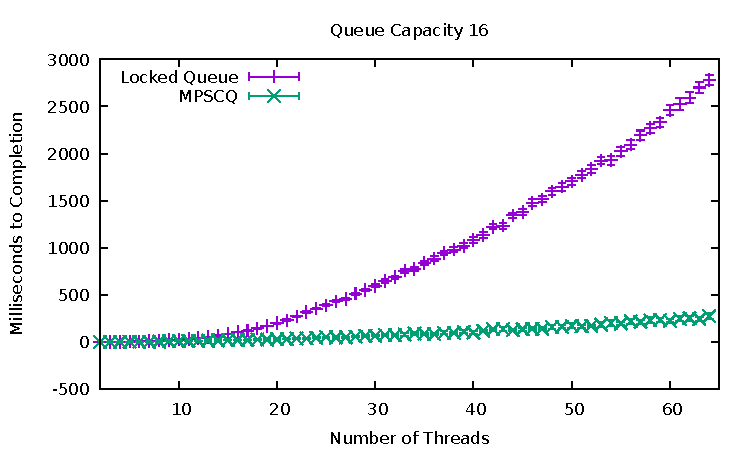
\includegraphics[width=170mm]{data_16.pdf}
	\caption{Average time to completion with varying number of threads for queue capacity 16.}
	\label{fig-16}
\end{figure}

Figure~\ref{fig-16} shows a very small queue capacity. This means that the queue
is immediately over-capacity. Here the wait-free queue does also experience
increasingly worse performance as the number of threads increases,
but the locked queue experiences much worse performance degradation and is
enormously slower when the number of threads is large.

\begin{figure}[h]
	\centering 
	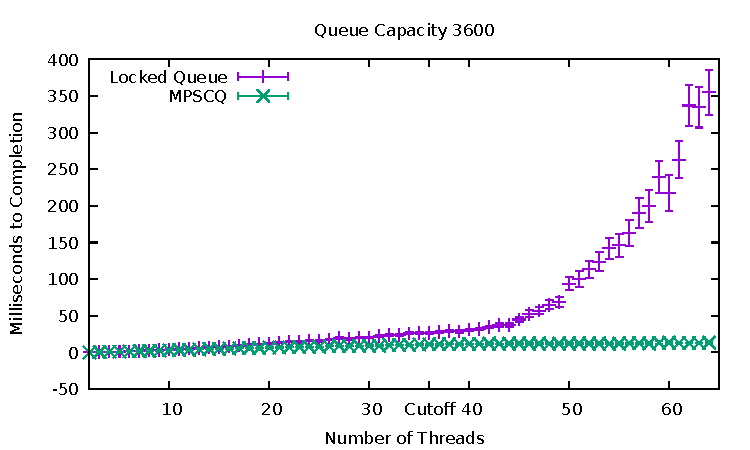
\includegraphics[width=170mm]{data_3600.pdf}
	\caption{Average time to completion with varying number of threads for queue capacity 3600.}
	\label{fig-3600}
\end{figure}

Figure \ref{fig-3600} shows a queue size that will have more capacity than necessary
until about halfway through the graph. At $n = 37$, there will be 36 producers
threads producing a total of 3600 items, which is the capacity of the queue.
Before this cutoff, the threads will always succeed in enqueuing an item.
There is still contention, and the performance of the locked queue is worse
due both to the overhead of the mutex and the thread contention. The wait-free
version acts much like a more performant version of the locked queue here.

Once the cutoff is reached, the wait-free queue quickly pulls ahead in
performance. The locked queue starts to exhibit exponentially increasing
time to completion as the number of thread increases, whereas the wait-free
queue remains seemingly unaffected and increases linearly. Both implementations
have to wait for the consumer thread to free up space in the queue before
a thread may enqueue something, but in the case of the locked queue the
consumer has to wait until it holds the mutex for the queue, whereas the
wait-free queue allows the consumer to always make forward progress, freeing
up space much more efficiently.

\begin{figure}[h]
	\centering 
	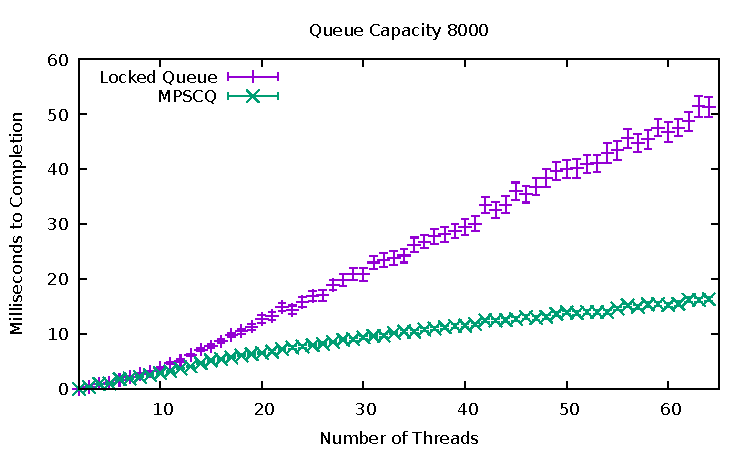
\includegraphics[width=170mm]{data_8000.pdf}
	\caption{Average time to completion with varying number of threads for queue capacity 8000.}
	\label{fig-8000}
\end{figure}

Figure \ref{fig-8000} shows a queue that has a capacity much larger than the
number of items to be enqueued with the maximum number of threads. Unlike
in figure \ref{fig-3600}, where this situation was hard to see in the first
half of the graph, this graph allows much closer examination of the differences
between the two implementations in the case where the producers do not need to
wait for the consumer thread to free up space. Both implementations appear
to exhibit linearly increasing time to completion as the number of threads
increases. However, the wait-free queue is still much more performant.

All three figures show similar performance of the two implementations when
the number of threads is very low. I believe that this is because the overhead
of starting threads and waiting until they join dominates the time required
for a small number of items to be processed by the producer and consumer threads.
Secondly, it appears that the wait-free implementation has much more stable
performance when compared to the locked queue, which is more susceptible to
the scheduling behavior of the operating system due to the blocking behavior
of mutexes.


\section{Conclusion}

The implementation of a wait-free multiple-producer single-consumer circular queue
was successful in significantly surpassing the performance of a similar locked queue in every way.
It has lower latency and better scalability, does not have the extra
overhead of a mutex, and has much more stable performance.
This will be a very useful addition to SeaOS, which has numerous
places where it uses a locked queue which could be replaced with this queue.

Keeping the codebase of SeaOS up to date with the C11 standards as they are
more and more supported has allowed me to drop a significant amount of complexity
from the codebase and gain new features, such as a more advanced atomic operations
library. Replacing the old atomics system in SeaOS with the one provided by
C11 allows me more control over the emitted code, and reduces the complexity
when porting the code to another platform.

\subsection{Future Work}

Looking forward, I plan to further reduce the ``lockiness'' of the kernel. There
are many places where locks are used due to convenience, but could be rewritten
so that they can synchronize safely using only atomic operations. Combined with
implementing more wait-free data structures, this will greatly improve the
operation of the kernel when many threads are operating inside of it.

Another ongoing piece of work is to
go through the codebase and relax the atomic operations that are currently
in use. This is a much more involved task, as reasoning about relaxed atomics
is even more challenging. Once the kernel is ported to platforms where the
relaxed atomics make a significant difference, I plan to compare the performance
of the kernel with and without the relaxation of the atomic operations to
determine if the extra complexity is worth it.

\vspace{10mm}

C11 atomics provide an excellent method of writing low-level atomic operations in
a higher-level language. They provide sufficient flexibility while abtracting
away the difficulties of dealing with concurrency such as reordering.
They are a good tool to understand more about how compilers
and processors allow threads to interact with each other and how to control them.
I was able to leverage C11 atomics to successfully implement a very fast wait-free
queue, which was a very enlightening first stab at wait-free data structures.
While it is understandable that the maintainers larger code bases, such as Linux,
would like to avoid keeping up with the advances of the language, I believe
that SeaOS's simplicity affords a unique opportunity to keep up with the changes
in the C programming language and explore the use of the new language features inside
of kernel space, hopefully improving maintainability and simplicity.


\clearpage

\bibliography{atomic}{}
\bibliographystyle{plain}

\end{document}

